%%%%%%%%%%%%%%%%%%%%%%%%%%%%%%%%%%%%%%%%%%%%%%%%%%%%%%%%%%%%%%%%%%%%%%%%%%%%%%%%%%%%%%%%%
% Section 8: Importing RSCPs and exporting TCPs
%	This section contains a description of the following:
%	- The contents of RapidSmith Checkpoints (RSCP)
% 	- How to load a RSCP into RapidSmith2 
%	- The contents of Tincr Checkpoints (TCP)
% 	- How to export a TCP from RapidSmith2 
%	- Important information that is imported from RSCP and how they are
% 		represented in RS2 (such as routethroughs) 	
%	- Code samples for importing RSCPs and exporting TCPs
%%%%%%%%%%%%%%%%%%%%%%%%%%%%%%%%%%%%%%%%%%%%%%%%%%%%%%%%%%%%%%%%%%%%%%%%%%%%%%%%%%%%%%%%%
\newpage
\section{Design Import/Export} \label{sec:import}
Importing and exporting designs between Vivado and RS2 is fairly
straightforward. It is done using RapidSmith Checkpoint (RSCP) and Tincr
Checkpoint (TCP) files, which contain a variety of information about a digital
design. This section describes in detail  the following: 

\begin{itemize}
  \item The contents of RSCP and TCP files
  \item How to load a RSCP into RS2, and how to export a RS2 design to a TCP
  \item Some additional information that is imported with a RSCP 
\end{itemize}

\subsection{RapidSmith Checkpoints}
RapidSmith checkpoints (RSCP) are Tincr checkpoints generated in Vivado from the
command \texttt{::tincr::write\-\_rscp}. These checkpoints are capable of
representing a Vivado design at any stage of implementation (post-synthesis,
post-place, and post-route), and can be parsed and imported into RapidSmith. As
we will see in \autoref{sec:tcp} below, the format of these checkpoints differ
slightly than those of regular TCPs. This is because a great deal of additional
information needs to be added to RapidSmith checkpoints in order to import a
complete representation of a Vivado design. The remainder of this subsection
describes each of the file types within a RapidSmith checkpoint, and what they
represent.

\subsubsection{design.info}
The \textit{design.info} file within a RSCP is used to include any useful
information about a design. Currently, it only stores the part name that the
design is implemented on. This file is reserved to add more additional
information in the future.

\subsubsection{netlist.edf}
The \textit{netlist.edf} file within a RSCP is an EDIF netlist representing the
logical portion of a design. It details all of the \cells, \nets,
and \ports within a design, and is generated from Vivado using the Tcl
command \texttt{write\_edif}. A RapidSmith \celldesign is created by parsing the
EDIF file, and converting it into the appropriate RS2 data structures described
in \autoref{sec:designDS}. Below is an example of a RSCP EDIF file.

\begin{lstlisting}[numbers=none, keywordstyle=, stringstyle=]
  (Library work
    (edifLevel 0)
    (technology (numberDefinition ))
   (cell add (celltype GENERIC)
     (view add (viewtype NETLIST)
       (interface 
        (port a (direction INPUT))
        (port b (direction INPUT))
        (port cin (direction INPUT))
        (port cout (direction OUTPUT))
        (port s (direction OUTPUT))
       )
       (contents
         (instance GND (viewref netlist (cellref GND (libraryref hdi_primitives))))
         (instance VCC (viewref netlist (cellref VCC (libraryref hdi_primitives))))
         (instance a_IBUF_inst (viewref netlist (cellref IBUF (libraryref hdi_primitives))))
         (instance b_IBUF_inst (viewref netlist (cellref IBUF (libraryref hdi_primitives))))
         (instance cin_IBUF_inst (viewref netlist (cellref IBUF (libraryref hdi_primitives))))
         (instance cout_OBUF_inst (viewref netlist (cellref OBUF (libraryref hdi_primitives))))
         (instance cout_OBUF_inst_i_1 (viewref netlist (cellref LUT3 (libraryref hdi_primitives)))
           (property INIT (string "8'hE8"))
         )
\end{lstlisting}

\subsubsection{placement.rsc}
The \textit{placement.rsc} file within a RSCP stores all of the placement
information of a Vivado design. This includes which package pin every \port is
mapped to, which \bel each \cell is placed on, and the logical-to-physical pin
mappings for each \cellpin. If a design has not yet been placed, this file
will be empty. Below is an example of a RSCP placement file.

\begin{lstlisting}[numbers=none]
LOC a_IBUF_inst R10 IOB33 INBUF_EN LIOB33_SING_X0Y50
PINMAP a_IBUF_inst O:OUT I:PAD 
LOC b_IBUF_inst T10 IOB33 INBUF_EN LIOB33_X0Y51
PINMAP b_IBUF_inst O:OUT I:PAD 
LOC cin_IBUF_inst T9 IOB33 INBUF_EN LIOB33_X0Y51
PINMAP cin_IBUF_inst O:OUT I:PAD 
LOC cout_OBUF_inst U13 IOB33 OUTBUF LIOB33_X0Y53
PINMAP cout_OBUF_inst O:OUT I:IN 
LOC cout_OBUF_inst_i_1 SLICE_X0Y51 SLICEL A6LUT CLBLL_L_X2Y51
PINMAP cout_OBUF_inst_i_1 O:O6 I0:A4 I1:A5 I2:A6 
LOC s_OBUF_inst T13 IOB33 OUTBUF LIOB33_X0Y53
PINMAP s_OBUF_inst O:OUT I:IN T:TRI 
PACKAGE_PIN R10 a
PACKAGE_PIN T10 b
PACKAGE_PIN T9 cin
PACKAGE_PIN U13 cout
PACKAGE_PIN T13 s
\end{lstlisting}

\subsubsection{routing.rsc}
The \textit{routing.rsc} file within a RSCP stores all of the routing
information of a Vivado design. This includes: 

\begin{itemize}
  \item The used \cls{Site} \cls{PIPs} within each \cls{Site} (which
  specifies the internal routing)
  \item A list of LUT \bels that are acting as static sources (see
  \autoref{sec:additionalInfo} for more details)
  \item A list of LUT \bels that are being used as routethroughs (see
  \autoref{sec:additionalInfo} for more details) 
  \item The name of each INTRASITE net
  \item The name, connecting \cls{SitePin}s, and used \cls{TileWire}s
  of each INTERSITE net.
  \item Special routing information for the VCC and GND nets.
\end{itemize}

\noindent
If Vivado has not yet been routed, this file will be mostly empty. Below is
an example of the contents within a RSCP routing file.

\begin{lstlisting}[numbers=none]
SITE_PIPS SLICE_X9Y80 SRUSEDMUX:0 CEUSEDMUX:IN COUTUSED:0 CLKINV:CLK DCY0:DX ...
SITE_PIPS SLICE_X13Y80 PRECYINIT:AX SRUSEDMUX:0 CEUSEDMUX:IN COUTUSED:0 ...
SITE_PIPS SLICE_X15Y80 SRUSEDMUX:0 CEUSEDMUX:IN COUTUSED:0 CLKINV:CLK DCY0:DX ...
SITE_PIPS M17 OUSED:0 

... 

STATIC_SOURCES SLICE_X2Y106/D6LUT/O6 SLICE_X2Y106/C6LUT/O6 SLICE_X4Y106/D6LUT/O6 ...
LUT_RTS SLICE_X5Y101/B6LUT/A6/O6 SLICE_X2Y100/A5LUT/A4/O5 SLICE_X5Y100/C6LUT/A6/O6 ...

...

INTRASITE AddSub[10]
INTERSITE AngStep1[0] SLICE_X2Y82/AX SLICE_X2Y87/AQ SLICE_X2Y84/A1
ROUTE AngStep1[0] CLBLM_R_X3Y87/CLBLM_M_AQ CLBLM_R_X3Y87/CLBLM_LOGIC_OUTS4 ...

...

VCC INT_L_X2Y107/VCC_WIRE INT_L_X2Y107/VCC_WIRE INT_L_X2Y107/VCC_WIRE ...
START_WIRES INT_L_X2Y107/VCC_WIRE INT_L_X2Y106/VCC_WIRE INT_R_X3Y106/VCC_WIRE ...
GND INT_R_X3Y106/GND_WIRE INT_R_X3Y106/GND_WIRE INT_R_X3Y106/GFAN1 ...
START_WIRES INT_R_X3Y106/GND_WIRE INT_L_X4Y106/GND_WIRE INT_R_X3Y105/GND_WIRE ...
\end{lstlisting}

\subsubsection{contraints.rsc}
The \textit{contraints.rsc} file within a RSCP stores all XDC constraints on a
Vivado design. XDC constraints are similar to UCF files for ISE designs. They
can be used to set the clock frequency, constrain a top-level port to a specific
package pin on the device, and set other physical implementation details. An
example of a RSCP constraints file can be seen below.

\begin{lstlisting}[numbers=none]
create_clock -period 5.000 -name sysClk -waveform {0.000 2.500}
set_property IOSTANDARD LVCMOS18 [get_ports clk]
set_property IOSTANDARD LVCMOS18 [get_ports ena]
set_property PACKAGE_PIN E15 [get_ports {Yin[12]}]
set_property PACKAGE_PIN H17 [get_ports {Xin[14]}]
set_property PACKAGE_PIN D18 [get_ports {Xin[7]}]
\end{lstlisting}

\noindent
As can be seen, a Vivado constraints file is essentially a list of Tcl commands
to execute before generating a bitstream. When importing a RSCP into RapidSmith,
each constraint is parsed into a \cls{XdcConstraint} object and stored in the
top-level \celldesign. Each \cls{XdcConstraint} has two fields, a String
command and a String representing all command arguments. \autoref{code:xdc}
demonstrates how to manipulate XDC constraints in RapidSmith. Future RS2 plans
include creating a more intelligent way of handling XDC constraints. 

\begin{lstlisting} [caption=How to manipulate XDC constraints in RS2,
label=code:xdc] 
// Getting a list of all constraints in the current design
List<XdcConstraint> xdcConstraints = design.getVivadoConstraints();

// Look for all of the "create_clock" constraints in the design
List<XdcConstraint> crtClks = xdcConstraints.stream()
                              .filter(xdc -> xdc.getCommandName().equals("create_clock")) 
                              .collect(Collectors.toList());

// Add a new XDC constraint to the design
XdcConstraint xdc = new XdcConstraint("set_property", "IOSTANDARD LVCMOS18 [get_ports clk]") 
design.addVivadoConstraint(xdc);
\end{lstlisting}

\subsubsection{macros.xml}

The \textit{macros.xml} file within a RSCP contains template information about
macro cells in a Vivado design that (a) were not fully flattened, and (b) do not
exist in the default Vivado cell library. Using the information in the XML file,
a \cls{LibraryCell} can be created and added to the \cls{CellLibrary} so that
the design can import correctly. More information about macro cells in
RapidSmith can be found in \autoref{sec:macros}.

\begin{lstlisting}[numbers=none]
<?xml version="1.0" encoding="UTF-8"?>
<root>
  <macros>
    <macro>
        <type>IOBUF</type>
        <cells>
            <internal>
                <name>IBUF</name>
                <type>IBUF</type>
            </internal>
            <internal>
                <name>OBUFT</name>
                <type>OBUFT</type>
            </internal>
        </cells>
        <pins>
            <pin>
                <name>IO</name>
                <direction>inout</direction>
                <type>MACRO</type>
                <internalConnections>
                    <pinname>IBUF/I</pinname>
                    <pinname>OBUFT/O</pinname>
                </internalConnections>
            </pin>
            ...
        </pins>
    </macro>
  </macros>
</root>  
\end{lstlisting}


\subsection{Tincr Checkpoints} \label{sec:tcp}
Tincr checkpoints are very similar to RapidSmith checkpoints, but they can be
used to import designs back into Vivado after they have been modified in
RapidSmith. The main different between TCPs and RSCPs, is that the
\textit{placement.rsc}, \textit{routing.rsc}, and \textit{constraints.rsc} files
turn into \textit{placement.xdc}, \textit{routing.xdc}, and \textit{constraints.xdc}
respectively. Vivado is able to parse the XDC files and apply physical
information to the design. On design export, RapidSmith produces
a TCP that is compatible with Vivado. The file formats of the three XDC files
will not be included in this documentation. If you are interested in their
format, the best way to learn is to consult the Vivado user guide and generate a
TCP from RapidSmith and view the individual files.

\subsection{Additional Information} \label{sec:additionalInfo}
The reason RSCP and TCP checkpoints are distinguished, is that there are
several design implementation aspects in Vivado that aren't explictly
represented. In order to accurately represent a design in RapidSmith, they
must be included somehow. This section describes the parts of the design that
aren't explicitly represented in Vivado, and how RapidSmith handles them.
\autoref{sec:importExportTcp} describes how to get a handle to the additional
information after a checkpoint has been imported.

\subsubsection{LUT Routethroughs}
Besides their use in implementing logic equations, LUT BELs can also act as
signal routethroughs. In Vivado, a LUT is marked as a  routethrough when its
configuration equation (CONFIG.EQN) maps the value of a single input pin
directly to the output pin. These LUTs are not explicitly represented in the
logical netlist because there is no cell placed on the corresponding BEL. 
\autoref{fig:routethroughs} shows two examples of LUTs in Vivado that are
configured as routethroughs.

\begin{figure}[h]
  \centering
  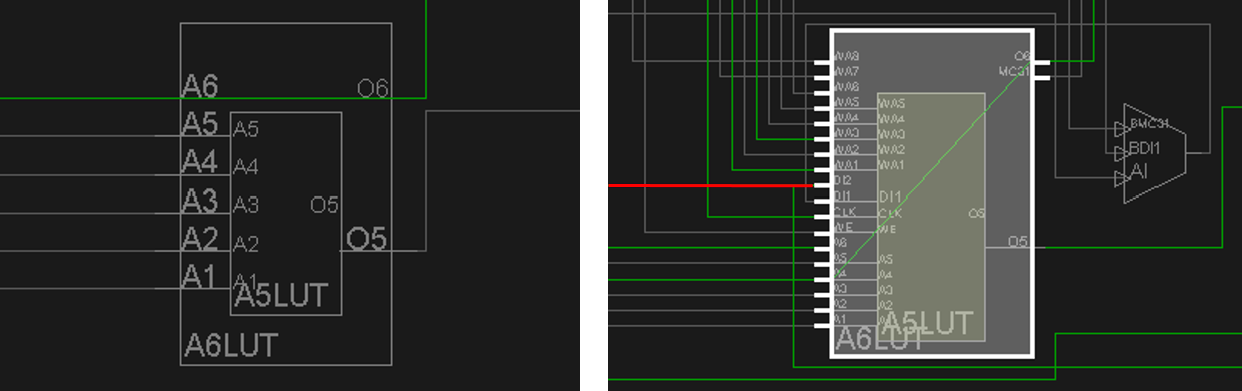
\includegraphics[width=1\columnwidth]{routethroughs}
  \caption{Two examples of LUTs being used as
  routethroughs in the Vivado GUI. The RT on the left uses the A6 input pin,
  while the RT on the right uses the A4 input pin. The net highlighted in red
  represents VCC.}
  \label{fig:routethroughs}
\end{figure}

\noindent
When a design is exported from Vivado, all LUTs that are acting as routethroughs
are included in the \textit{routing.rsc} file of a RSCP. When the file is
parsed, each routethrough is stored in a \cls{BelRoutethrough} object which
contains the physical \bel, the input \belpin, and the output \belpin that
uniquely describes the routethrough. It is important to note that if a \bel is
being used as a routethrough, no \cell can be placed there. When creating CAD
tools, \cls{BelRoutethrough}s give the user a more complete picture of what
\bels are actually available. 
	
As described in \autoref{otherConns}, there is a \cls{Connection} object in
RapidSmith from every input LUT pin to the LUTs output pin. These \bel
routethrough connections, are actually just \cls{WireConnection}s with the
\texttt{isRoute\-through()} method returning true. In order to use a LUT as a
routethrough in RapidSmith, you simply have to include the corresponding
\cls{WireConnection} within an INTRASITE \cls{RouteTree}. When a design is
exported from RapidSmith, the routethrough \cls{WireConnection}s are
automatically detected and converted to a passthrough LUT \cell. The netlist
is rewired appropriately.

\subsubsection{Static Source LUTs}
LUTs can also act as a static power or ground source. This occurs when the
configuration equation is set to 1 or 0. An example of a LUT that exhibits
this behavior is shown in \autoref{fig:staticSourceLut}. When a design
is exported from Vivado, all LUTs that are acting as static sources are
included in the \textit{routing.rsc} file of a RSCP. As the file is being
parsed, a list of static sources \bels are recorded and stored in a list data
structure. Just like routethroughs, if a \bel is being used as a static source
no \cell should be placed on it.

\begin{figure}[h]
  \centering
  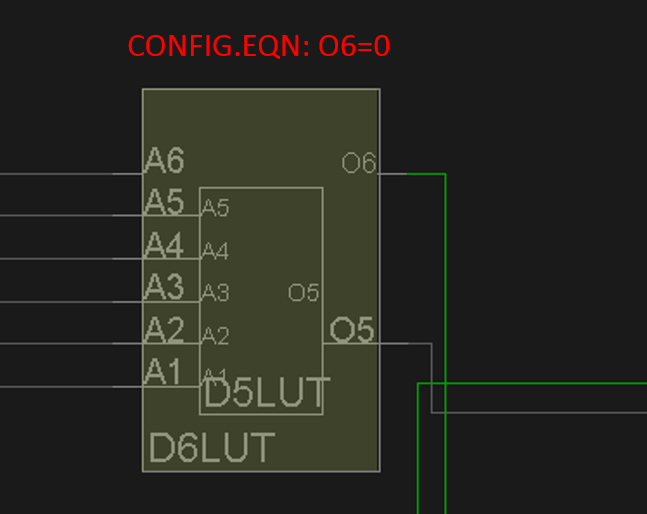
\includegraphics[width=.5\columnwidth]{staticSourceLut.png}
  \caption{A LUT \bel that has been configured as a GND source. Notice that
  there are no input pins being driven.}
  \label{fig:staticSourceLut}
\end{figure}

\subsubsection{Pseudo CellPins}
\cls{PseudoCellPin}s are described in great detail in \autoref{sec:cellPin}.
When a RSCP is loaded, \cls{PseudoCellPin}s are automatically detected,
created, and attached to their corresponding \cells.

\subsection{Importing RSCPs and Exporting TCPs} \label{sec:importExportTcp}
After a Vivado design has been converted to a RSCP using the
\texttt{::tincr::write\_rscp} command, it can be loaded into RapidSmith.
\autoref{code:import} demonstrates the basix syntax of design
import and export.

\begin{lstlisting}[caption=How to import and export TCP files to and from RS2,
label=code:import]
// Loading a Tincr Checkpoint
TincrCheckpoint tcp = VivadoInterface.loadTcp("pathToCheckpoint.tcp");
CellDesign design = tcp.getDesign();
Device device = tcp.getDevice();
CellLibrary libCells = tcp.getLibCells();

// Insert CAD Tool Here

// Exporting the modified design to a Tincr Checkpoint
VivadoInterface.writeTCP("pathToStore.tcp", design, device, libCells);

\end{lstlisting}

\noindent
While a design is being imported into RapidSmith, several useful data structures
are built up. If you want to gain access to those data structures, you can pass
an additional argument into the \texttt{VivadoInterface.loadTCP} method. This
is shown in \autoref{code:import2}.

\begin{lstlisting}[caption=Importing a TCP with additional information,
label=code:import2]
// Loading a Tincr Checkpoint with additional info
TincrCheckpoint tcp = VivadoInterface.loadTcp("PathToCheckpoint.tcp", true);
Collection<BelRoutethrough> belRts = tcp.getRoutethroughObjects();
Collection<Bel> staticSources = tcp.getStaticSourceBels();
Map<BelPin, CellPin> belPinToCellPinMap = tcp.getBelPinToCellPinMap()
\end{lstlisting}

\noindent
After a design is exported from RapidSmith, a Tincr Checkpoint (TCP) is
produced. To import the TCP back into Vivado, simply open up Vivado in Tcl mode
and use the following command:

\begin{code}
Vivado% tincr::read_tcp myCheckpoint.tcp
\end{code}